%%% Local Variables:
%%% mode: latex
%%% TeX-master: t
%%% End:


\documentclass{article}
\usepackage[T1]{fontenc}
\usepackage[utf8]{inputenc}
\usepackage{amsmath}
\usepackage{amssymb}
\usepackage{hyperref}
\usepackage{parskip}
\usepackage{float}
\usepackage{graphicx}
\usepackage{listings}
\usepackage{cleveref}
\usepackage{circuitikz}
\usepackage{listings}

\title{Design of Digital systems 1 TFE4141 - Assignment 4}
\author{Sindre Hansen - 732719}
\date{Fall 2016}

\renewcommand\thesection{\arabic{section}}
\renewcommand\thesubsection{\thesection.\arabic{subsection}}


\begin{document}
\begin{figure}
  \centering
  
\includegraphics[width=0.5\textwidth]{images/logontnu_eng}
\end{figure}
\maketitle
\rule{\linewidth}{0.5mm}

\section{Task 1}
\subsection{}
\begin{figure}[hbp]
  \centering
  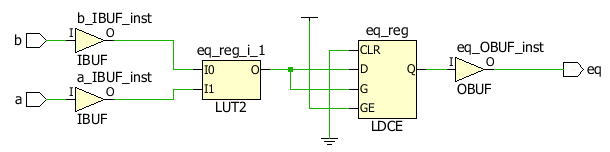
\includegraphics[width=\textwidth]{images/task1-1}
\end{figure}

\subsection{}
An example where a latch is unintentionally created is when you don't
assign values to all output in every branch of an if-statement.

\subsection{}
The way to make sure that latches are not generated from combinatorial
processes is to always make sure that there are no incomplete
branches, or incomplete signal assignments.

\section{Task 2}
\subsection{}
If we assume that on the first run the reset is held high then there's
created a single flip-flop for 't' in both designs. However, if we on
the next run assume that the reset is low, the difference in the two
designs become clearer. Since design1 has the signal assignment before
the variable assignment it needs to create another flip-flop for
't'. Therefore we end up with two flip-flops in the synthesis.

Design2 has the signal assignment after the variable assignment and
therefore we end up with just one flip-flop in the synthesis.

\subsection{}
Image: task2-design1

Image: task2-design2

\subsection{}





\end{document}
